\chapter{How congestion shapes cities}

Empirical evidence suggest that most urban systems experience a
transition from a monocentric to a polycentric organisation as they
grow and expand. We propose here a stochastic, out-of-equilibrium model of the
city which explains the appearance of subcenters as an effect of
traffic congestion. We show that congestion triggers the unstability
of the monocentric regime, and that the number of subcenters and the
total commuting distance within a city scale sublinearly with its
population, predictions which are in agreement with data gathered for
around 9000 US cities between 1994 and 2010.\\


As cities grow, they evolve from a monocentric organisation where all
the activities are concentrated in the same geographical area
--usually the central business district-- to a more distributed,
polycentric organisation~\cite{Kemper:1974,Odland:1978,Mills:1972,Griffith_PG:1981,Dokmeci:1994,McMillen:2003,Pereira:2013,Roth:2011}.  We present in this Letter a stochastic, out-of-equilibrium model of the
city which relies on the assumption that the polycentric structure of
large cities might find its origin in congestion, irrespective of the
particular local economic details. We are able to reproduce many
stylized facts, and --most importantly-- to derive a general relation
between the number of activity centers of a city and its
population. Finally, we verify this relation against the employment
data from around 9000 cities in the US between 1994 and 2010.

%\section{The model}


\section{Fujita and Ogawa}
\label{sec:fujita_and_ogawa}

In line with the tradition of economic geography~\cite{Fujita:2001}, the model
of Fujita and Ogawa~\cite{Fujita:1982} is based on the concept of agglomeration
economies---to explain why economical activities tend to group---and the spatial
distribution of wages and rents across the urban space. They consider that
cities are constituted of two kinds of actors: the firms, who tend to
concentrate to maximise their production, and the households, who try to
minimise their rent and commuting cost. In the following, I will present the
model, focusing on the hypotheses.\\ 

The model is \emph{static}, in the sense that the number of firms and
individuals are fixed. It is an \emph{equilibrium} model, considering the the
city is the realisation of a general optimum. The original model is also
\emph{one-dimensional}, although the hypothesis of one-dimensionality is not
fundamental, and only necessary to make the calculations easier. Because I will
not try to solve the model, I will write equations in the 2D case.

\subsection{Households} 
\label{sub:households}

Fujita and Ogawa assume that there is a fixed number $N$ of households in the
city. The households are considered identical, in the sense that they all have
the same utility function and the same budget constraint. The utility function
of each household is given by the function $U = U(Z)$ where $Z$ is the surplus
of money that is left after budgetary constraints (expressed in monetary units).
Basically the money one has left at the end of the month, once the rent, bills
and petrol (or transportation card) are paid. 

The utility is assumed to be an increasing function of $Z$ so

\begin{equation}
    \frac{\partial U}{\partial Z} > 0
\end{equation}

The budget constraint on an household living at $i$ (of coordinates $\vec{x}$)
and working at the firm located at $j$ (of coordinates $\vec{y}$) is given by the
equation

\begin{equation}
    Z = W\left(j\right)
      - C_R\left(i\right)
      - C_T\left(i,j\right)
\end{equation} 

where $W\left(j\right)$ is the wage earned at $j$, $C_R\left(i\right)$ the total
rent paid at $i$ and $C_T\left(i,j\right)$ the cost of commuting between
home and work. This equation is very general, and will be our starting point for
the model presented in the next section. The authors of~\cite{Fujita:1982}
further specify the commuting cost

\begin{equation}
    C_T\left(i,j\right) = t\,d_E(i,j) = t\,\left|\vec{y}-\vec{x}\right|
\end{equation}

where $t$ the commuting cost per unit distance, and $d_E(i,j) = \left| \vec{y} -
\vec{x} \right|$ the euclidean distance between home and work. The total rent
cost is further written as

\begin{equation}
    C_R\left(i\right) = R(i)\,S_h
\end{equation}

where $R(i)$ is the rent per unit surface at $i$, and $S_h$ the surface area
used by households, which becomes a parameter of the model.
The surplus $Z$
finally reads

\begin{equation}
    Z = W\left(j\right)
      - R\left(i\right)\,S_h
      - t\,d_E\left(i,j\right)
\end{equation} 


\subsection{Firms}
\label{sub:firms}

The second type of agents taken into consideration in the model are the firms.
It is assumed that all firms employ the same number of individuals, which
amounts to having a fixed number of firm $M$ (once the number of households is
fixed). The profit earned by a firm  located at $j$ reads, in a general
form

\begin{equation}
    \Pi = G\left(j\right) 
        - C_R\left(j\right) 
        -  W\left(j\right)\,L_f
\end{equation}

where $G$ is the total gain realised by the firm selling its production, $C_R$
the rent paid by the firm, and $L_f$ the total number of employees per firm---a
paramter of the model.\\

To take agglomeration economies into account, Fujita and Ogawa define the
locational potential $F$ defined by

\begin{equation}
    F\left(j\right) = \int_{\mathcal{C}} b(\vec{x})\,e^{-\alpha\,\left|\vec{y}-\vec{x}\right|}\:\mathrm{d}\vec{x}
\end{equation}

where $b(\vec{x})$ is the density of firms at $\vec{x}$. The integral runs over
the entire city's spatial extent $\mathcal{C}$. One can easily see that the
higher the density of firms in a radius of $1/\alpha$ around a firm, the higher
the locational potential is going to be. Balanced by the constraint imposed by
the rent, which prevents too many firms from agglomerating at the same location,
the locational potential likely is the term responsible for the existence of
polycentric solutions in the model. Indeed,the authors further write the total
gain $G$ as a multiple of $F$:

\begin{equation}
    G(j) = \beta\,F(j)
\end{equation}

where $\beta$ integrates both the productivity of the employees and the effect
of the locational potential. The rent, as
in the case of households, is written $C_R(j) = R(j)\,S_f$ where $S_f$, the
surface needed by firms, is a parameter of the model. The profit
of companies therefore reads

\begin{equation}
    \Pi = \beta\, \int_{\mathcal{C}} b(\vec{x})\,e^{-\alpha\,\left|\vec{y}-\vec{x}\right|}\:\mathrm{d}\vec{x}
        - R\left(j\right)\,S_f
        - W\left(j\right)
\end{equation}


\subsection{Equilibrium conditions and results}
\label{sub:equilibrium_conditions}

Once the budget constraints have been explicited, one needs to further define
the equilibrium conditions to be able to solve the model. First, the goal of
each household is to maximise their utility under the budget constraint.\\

[Explicit calculations here]\\

In other words, the maximisation of utility under budget constraints is
equivalent to chosing the residential location $i$ and the job location $j$ so
as to maximise $Z$. In other words, the maximisation of utility in this
particular is equivalent to performing a cost-benefit analysis. The firms have
no utility function, and choose to be a the location $j$ that maximises their
profit.\\

A further constraint is given by the bid-rent curve and goes as follows. The authors define two intermediate functions, $\Psi(\vec{x})$ and $\Phi(\vec{x})$ which are
respectively the bid rent function of households and of firms, defined as

\begin{align}
    \Psi\left(\vec{x}\right) &= \max_{\vec{x}} \left\{ \frac{1}{S_h} \left[W(\vec{x} ) - Z -
    t\,d_E\left(\vec{x}-\vec{y}\right)\right] | U(Z)\right\}\\
    \Phi\left(\vec{x}\right) &= \frac{1}{S_f} \left[\beta\,F(\vec{y}) - \Pi -
W(\vec{y})\right]
\end{align}

$\Psi(\vec{x})$ represents the maximum rent that the households could pay to be
located at $\vec{x}$ while still having a utility value $U$. $\Phi(\vec{y})$ is
the maximum rent that firms could pay to be located at $\vec{y}$. At
equilibrium, it is assumed that whoever's bid rent function is maximum at
$\vec{x}$ will be located at $\vec{x}$.\\

The results of this model, given its intricacy, are somewhat disapointing.
Unsurprisingly, the authors are not able to derive an analytical solution for
their model. What they do, however, is deriving the conditions on the parameters
for the existence of monocentric and polycentric organisations of activities,
using numerical methods.

\section{Problems with the Fujita and Ogawa model}
\label{sec:problems_with_the_fujita_and_ogawa_model}

This approach fails at giving a satisfactory quantitative account  of the
polycentric transition of cities. A lot can be said about the details of the
model and its assumptions. We choose here to only discuss the issues that we
feel are the most important, and that we will try to adress in our model. 

\paragraph{It is an equilibrium model.} In line with the rest of Urban
Economics~\cite{Fujita:2001, Fujita:2013}, they describe a city as being in
an equilibrium characterised by static spatial distributions of households and
business firms. However, the equilibrium assumption is unsupported as cities are
out-of-equilibrium systems and their dynamics is of particular interest for
practical applications~\cite{Batty:2008}.\\

\paragraph{It is too complex.} It integrates so many interactions and
variables that it is difficult to understand the hierarchy of processes
governing the evolution of cities, which ones are fundamental and which ones a
irrelevant. A model is only interesting when it
provides a simple structure to understand empirical results, whether it
reproduces them, or provides well-understood limiting case.\graffito{Limiting
case models are often called `null models'} 

\paragraph{It does not make any prediction.} Worse, due to its complexity, the
model is unsolvable, and does not make any prediction. At best it shows that
polycentric configurations are \emph{possible}. Yet, there are possibly different
models[possibly? Loo
at literature in economics] that admit polycentric activity profiles as a
solution. The model is thefore unsupported by data.\\ 

We also note that the model does not take the congestion into account in the
commuting cost (which is only a function of the distance). However, it is
mentioned in the economics literature as being a possible cause of the
polycentric transition of cities~\cite{McMillen:2003}. 

\section{Modeling the polycentric transition}
\label{sec:an_out_of_equilibrium_model_}

Following recent interdisciplinary efforts to construct a quantitative
description of cities and their
evolution~\cite{Makse:1995,Zanette:1997,Marsili:1998a,Marsili:1998b,Batty:book2005,Bettencourt:2007,Batty:2008},
we deliberately omit certain details and focus instead on basic processes. We
thereby aim at building a minimal model which captures the complexity of the
system and is able to account for --qualitative as well as quantitive-- stylized
facts. 
The model we propose is by essence dynamical and describes the evolution
of cities' organisation as their population increases. We focus on car
congestion -- mainly due to journey-to-work commutes -- and its effect on the job
location choice for individuals.\\

\subsection{Decoupling the choice of household and job}
\label{sub:decoupling_the_choice_of_household_and_job}

The time scales involved in the evolution of cities are usually such that the
employment turnover rate is larger than the relocation rate of households. On a
short time scale, we can thus focus on the process of job-seeking alone, leaving
aside the problem of the choice of residence. In other words, we assume the
coupling between both processes to be negligible: we assume that each inhabitant
newly added to the city has a random residence location and we concentrate on
understanding how such an inhabitant chooses its job location.\\

As a result of this assumptions, a worker living at $i$
will choose to work at the center $j$ such that the quantity
 
\begin{equation}
    Z_{ij} = W(j) - C_T(i,j)
    \label{eq:Z_workers_general}
\end{equation}

is maximum. Doing so, we give up any hope to describe the spatial structure of the rent
distribution, or the alledged scaling between rent prices and population size in
cities.

\subsection{Decoupling the dynamics of residence and work locations}
\label{sub:decoupling_the_dynamics_of_}

Another difficulty with the Fujita-Ogawa model is the strong coupling between
the behaviour of firms and individuals. The empirical literature on the
behaviour of firms points to a tendency of similar industries to cluster
geographically~\cite{Marcon:2003, Duranton:2005, Marcon:2009}, and a higher
profit of industries located in Urban environments~\cite{Melo:2009}. Although
theoretical attempts at explaining these behaviours have been
proposed~\cite{Duranton:2004}, the models are yet to be developped in an
out-of-equilibrium framework.\\

Here, we decide to simplify the problem by assuming that firms indeed cluster
into specific locations, that we call activity centers. Each worker can then
choose among a pool of $N_c$ potential activity centers (which we suppose are
also randomly distributed among the city). The active subcenters are then
defined as the subset of potential centers which have a non zero incoming number
of individuals. We thus assume that the existence of activity centers is defined
by the willingness of workers to work in the possible locations.\\


We now discuss the form of the wage $W(j)$ and the commuting cost $C_T$ that are
present in equation~\ref{eq:Z_workers_general}. 

\subsection{Determining the wage}
\label{sub:determining_the_wage}

The problem of determining the (spatial) variations of the average wage $W(j)$
at location $j$ is very reminiscent of some problems encountered in fundamental
physics. Indeed, the wage depends on many different factors, ranging from the
type of company, the education level of the inhabitant, the level of
aglomeration, etc., and in this respect is not too different from quantities
that can be measured in a large atom made of a large number of interacting
particles. In this situation, physicists found out that although it is possible
to write down the corresponding equations, not only is it impossible to solve
them, but also not really useful. In fact they found out~\cite{Dyson:1962} that
a statistical description of these systems, relying on random matrices could
lead to predictions which agree with experimental results.\\

We wish to import in spatial economics this idea of replacing a complex quantity
such as wages --which depends on so many factors and interactions-- by a random
one. The problem is not so much that we cannot write down the equations that
determine the wage that an individual could get in a given company. Even if we
could, the sheer number of people living in a urban area would surely prevent us
from solving these equations. And even if we could solve them, the resulting
information would be too overwhelming to really allow us to understand the
large-scale behaviour of the system as a whole. We thus need an \emph{effective}
theory of cities.
We therefore decide to account for the interaction between activity centers
and people by taking the wage as proportional to a random variable $\eta_j \in
\left[ 0,1\right]$ such that $W(j) = s\, \eta_j$ where $s$ defines the maximum
attainable average wage in the considered city.\\

We are aware that wages are not determined endogeneously but is rather the
result of thousands, millions of interactions between firms and individuals. In
the same way that Dyson did not mean that the interactions between electrons in
large atoms \emph{are} random, our assumptions does not mean that wages are
intrisincally randomly determined. What we mean, however, is that in the case of
systems containing a large number of individuals, one may possibly do \emph{as
if} they were randomly determined. Although we thereby abandon the possibility
to describe the dynamics of the wage distribution and the spatial 

\subsection{Commuting cost and congestion}
\label{sub:the_commuting_cost}


As for the transportation cost $C_T(i,j)$, we choose it to be
proportional to the commuting time between $i$ and $j$. In a typical
situation where passenger transportation is dominated by personal
vehicles, this commuting time not only depends on the distance between
the two places, but also on the traffic between $i$ and $j$, the vehicle capacity of
the underlying network and its resilience to congestion. The Bureau of
Public Road formula~\cite{Branston:1976} proposes a simple form taking
all these ingredients into account. In our framework, it leads to the following expression for the 
commuting costs

\begin{equation}
    C_T(i,j) =  t\, d_{ij} \left[ 1 + \left( \frac{T_{ij}}{c} \right)^{\mu} \right]
    \label{eq:commuting_cost}
\end{equation}

where $T_{ij}$ the trafic per unit of time between $i$ and $j$ and $c$
is the typical capacity of a road (taken constant here). The quantity
$\mu$ is a parameter quantifying the resilience of the transportation
network to congestion. We further simplify the problem by assuming
than the traffic $T_{ij}$ is only a function of the subcenter $j$ and
therefore write $T_{ij}=T(j)$ the total traffic incoming in subcenter
$j$ (see Supplementary Material~\cite{SM} for a short discussion).

\subsection{Summary}
\label{sub:summary}


In summary, our model is defined as follows. At each time step, we add
a new individual $i$ located at random in the city, who will
choose to work in the activity area $j$ (among $N_c$ possibilities
located at random) such that the following quantity
%
\begin{equation}
Z_{ij} = \eta_j - \frac{d_{ij}}{\ell} \left[ 1 + \left( \frac{T(j)}{c} \right)^{\mu} \right]
\label{eq:cost_function}
\end{equation}
%
is maximum (we omitted irrelevant multiplicative factors). The quantity $\ell = s/t$ is interpreted as the maximum effective
commuting distance that people can financially withstand. 

\subsection{Monocentric to polycentric transition}
\label{sub:monocentric_to_polycentric_transition}

Depending on the relative importance of wages, distance and congestion, the
model predicts the existence of three different regimes: the monocentric regime
(top left Fig.~\ref{fig:model_results}), the distance-driven polycentric (top
right Fig.~\ref{fig:model_results}) regime and the attractivity-driven
polycentric (bottom Fig.~\ref{fig:model_results}) regime. 


\begin{figure}
    \centering
    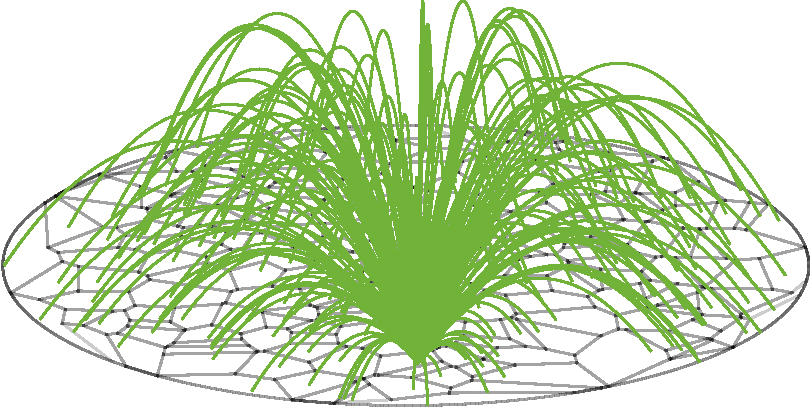
\includegraphics[width=0.49\textwidth]{gfx/chapter-monocentric/1.pdf}
    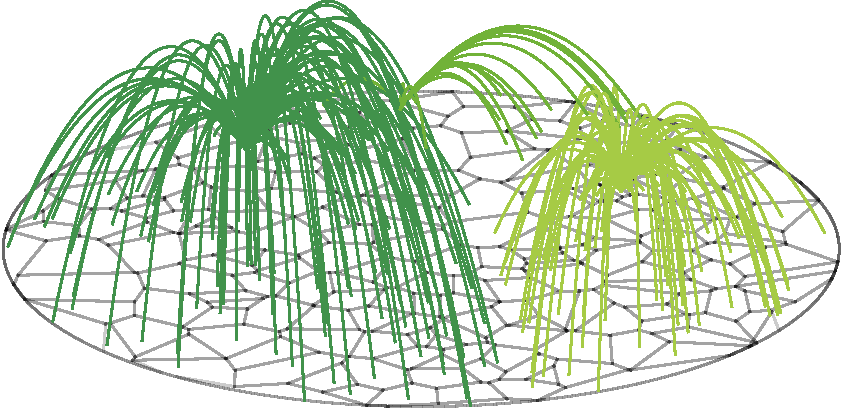
\includegraphics[width=0.49\textwidth]{gfx/chapter-monocentric/2.pdf}
    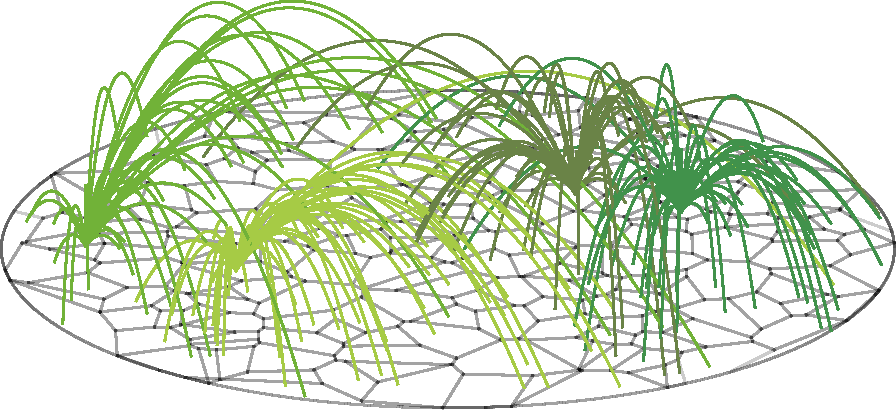
\includegraphics[width=0.49\textwidth]{gfx/chapter-monocentric/3.pdf}
    \caption{The monocentric (top left), distance-driven polycentric (top right)
      and attractivity-driven polycentric (bottom) regimes as produced by
      our model. Each link represents a commuting journey to an activity center. \label{fig:model_results}}
\end{figure}

The existence of a monocentric regime depends on how $\ell$---the maximum commuting distance that people can
afford--- compares to the size of the city $L$. Indeed, it is easy to
see that people located at a distance $d_{ij} > \ell$
from the most attractive center will not be able to afford commuting to this
center, and will, according to our model, choose to commute to a closer center.
As a result, a monocentric regime is only sustainable as long as people's
residence is drawn close to the most attractive center. In the limit where $\ell
\gg L$, the attractiveness of a center becomes irrelevant, and a monocentric regime cannot
exist. In these cases, we end up in the situation shown on the top-right of
Fig.~\ref{fig:model_results}.\\


From now on, we will assume that $\ell$ is large enough so that a
monocentric state exists for small values of the population. In this
regime, the value of $\eta$ prevails and the monocentric state evolves
to an attractivity-driven polycentric structure as the population
increases. 
Starting from a small city with a monocentric
organisation, the traffic is negligible and 

$$Z_{ij}\approx \eta_j$$

which implies that all individual are going to choose the most attractive
center, that is the center with the largest value of $\eta_j$, say $\eta_1$.
When the number $P$ of households increases, the traffic will also increase and
some initially less attractive centers (with smaller values of $\eta$) might
become more attractive, leading to the appearance of new subcenters
characterized by a non-zero number of commuters. More specifically, a new
subcenter $j$ will appear when for an individual $i$, we have 

$$Z_{ij}>Z_{i1}$$

Because we assume we were in a monocentric state, the traffic so far is such
that $T(1)=P$ and $T(j)=0$ which leads to the equation

\begin{equation}
    \eta_j-\frac{d_{ij}}{\ell}>\eta_1-\frac{d_{i1}}{\ell}\left[1+\left(\frac{P}{c}\right)^\mu\right]
\end{equation}

We assume that there are no spatial correlations in the subcenter distribution,
so that we can make the approximation $d_{ij}\sim d_{i1}\sim L$. The new
subcenter will thus be such that $\eta_1-\eta_j$ is minimum implying that it
will have the second largest value denoted by $\eta_j=\eta_2$. 

According to order statistics, we have on average for a uniform distribution

$$\overline{\eta_1-\eta_2}\simeq 1/N_c$$

hence a critical value for the population

\begin{equation}
    \boxed{P^*= c \left( \frac{\ell}{L N_c} \right)^{1/\mu}}
    \label{eq:critical_population}
\end{equation}

Whatever the system considered, there will \emph{always} be a critical
value of the population above which the city becomes polycentric. The
monocentric regime is therefore fundamentally unstable with regards to
population increase, which is in agreement with the fact that no major city in
the world exhibits a monocentric structure. We note that the smaller the value
of $\mu$ (or larger the value of the capacity $c$), the larger the critical
population value $P^*$ which means that cities with a good road system capable
of absorbing large traffic should display a monocentric structure for a longer
period of time.

\section{Number of centers}
\label{sec:number_of_centers}


We have so far established that, because of increased levels of congestion as
the population grows, all cities will eventually adopt a polycentric
structure. Although appealing and in agreement with a common observation, the
prediction given by Eq.~\ref{eq:critical_population} is impossible to test with
the currently available data. Therefore, we would like to compute what the model
predicts for the variation of the number of subcenters with population.\\

We compute the value of the population at which 
the $k^{th}$ center appears. Still in the attractivity-driven regime, we assume
that so far $k-1$
centers have emerged with 

$$\eta_{1} \geq \eta_{2} \geq \ldots \geq \eta_{k-1}$$

with a number of commuters $T(1), T(2), \ldots,
T(k-1)$, respectively. The next worker $i$ will choose the center $k$ if

\begin{equation}
    Z_{ik} > \max_{j \in \left[1,k-1\right]} Z_{ij}
\end{equation}

which reads

\begin{equation}
    \eta_k - \frac{d_{ik}}{\ell} > \max_{j \in \left[1,k-1\right]} \left\{
    \eta_j - \frac{d_{ij}}{\ell} \left[ 1 + \left(
      \frac{T(j)}{c}\right)^\mu\right] \right\}
\end{equation}

According to simulations of the model, we know that the distribution of traffic $T(j)$ is
narrow, and we can assume that all the centers have roughly the same number of
commuters $T(j) \sim P/(k-1)$. As above we also assume that there are no spatial
correlations in the position of employment centers so that $d_{ij} \sim d_{ik} \sim L$. 
We can now write the previous expression as


\begin{equation}
\frac{L}{\ell} \left( \frac{P}{(k-1)\,c} \right)^{\mu} > \max_{j \in
  \left[1,k-1\right]} \left( \eta_j \right) - \eta_k
\end{equation}
Following our definitions, $\max_{j \in \left[1,k-1\right]} \left(
\eta_j \right) = \eta_1$. According to order statistics, if the
$\eta_j$ are uniformly distributed, we have on average
$$\overline{\eta_1 - \eta_k} = (k-1)/(N_c+1)$$ 

It follows from these assumptions that (1) the $k^{th}$ center to appear is the
$k^{th}$ most attractive one (2) the average value of the population
$\overline{P}_k$ at which the $k^{th}$ center appears is given by:

\begin{equation} 
    \overline{P}_k = P^* \left( k-1 \right)^{\frac{\mu+1}{\mu}}
\end{equation}

Conversely, the number $k$ of subcenters scales sublinearly with population as

\begin{equation} 
    \boxed{k \sim \left( \frac{P}{P^*} \right)^{\frac{\mu}{\mu
    + 1}}}
    \label{eq:centers_prediction}
\end{equation} 

For positive values of $\mu$, we have $\frac{\mu}{\mu+1}<1$. we can thus
conclude that the number of activity subcenters in urban areas scales sublinearly
with their population where the prefactor and the exponent depend on the
properties of the transportation network of the city under consideration. 

[Link to the empirical observations]

\section{Conclusion}
\label{sec:conclusion}

Before concluding on the merits of the model and what we learn from it, and to
avoid mis-interpretations of its conclusions, it is necessary to state what the
model does not say and to present its limits.

\subsection{What the model does not say}
\label{sec:what_the_model_does_not_say}

\graffito{This discussion owes largely to questions raised during presentations
of this work.}

A first feature, hidden in the assumptions of the model, is that it does
not explain the concentration of activities in localised areas in the cities.
Rather, it takes the existence of centers as granted, and does not bother with
the behaviour of firms. Thereby, we do not pretend to explain the complexity of
urban dynamics in its entirety, but rather a single aspect of it. Of course,
this is a topic worthy of investigation, and should be studied seriously is one
wants to have a comprehensive understanding of the mechanisms that shape cities.

A second limitation lies in the description of congestion. In a worry of
simplificating the problem, we chose to adopt a macro-scale description of
traffic congestion, given by Eq.~\ref{eq:commuting_cost}. The sensitivity of the
road network to congestion is taken into account through the exponent $\mu$ and
the capacity $C$, which are assumed to be the same across the entire city. A
full specification of these parameters would need to understand how local
patterns of congestion lead to macroscropic behaviours at the city scale.  This
is, of course, a difficult entreprise:  local particularities of the layout may
have dramatic consequences on the fluidity of traffic, and congestions do
propagate through the network so that access to a given center can have an
effect on the travel to another center. 

\subsection{A predictive model}
\label{sub:a_predictive_mode}

The model we just presented, although not perfect, exhibits some of the
desirable features of a model we presented in the introduction. First, it goes
beyond the standard models in urban economics by going beyond the explanation of
stylized facts. As we saw earlier, one major problem with the model of Fujita
and Ogawa is the absence of quantitative prediction. Instead of providing a
prediction that can be further confirmed or refuted by empirical observation,
the authors merely tested the existence of polycentric solutions in the
framework of their model. The link with reality is however very loose, in the
sense that there is a big intellectual leap between the actual prediction of the
model and reality. Even though the model proposed here is very simple, it is not
difficult to link it to reality. Once the notion of activity centers is defined
empirically, it is not difficult to count this number of centers and look at the
dependence of this number on the population size of the considered city. The
model can then be confirmed, or refuted. Furthermore, as we will see in the
following section, the model serves as a basis to the understanding of some of
the scaling relationships in cities, linking the model even more strongly to the
empirical reality.

\subsection{Understanding the polycentric transition}
\label{sub:understanding_the_polycentric_tranistion}

Second, the model allows us to \emph{understand} why the polycentric transition
occurs. Taking a step back on the assumptions that led to the prediction of
Eq.~\ref{eq:centers_prediction}, one can see that what triggers the transition
in our model is the congestion term in Eq.~\ref{eq:cost_function}. The positions
of households and firms are indeed taken as random, the wages are also taken at
random. Therefore, we can conclude that our model explains the polycentric
transition of cities through the increasing congestion around employment centers
as the population increase. More mechanisms probably are involved, but the model
shows that congestion alone is enough to lead to a polycentric situation while
the population increases.\\

If we assume that agglomeration economies is the basic process explaining the
existence of centers in the first place, the model brings evidence that this
centripetal force is balanced by the centrifugal effect of congestion, that
tears city apart. Arguably, the non trivial spatial patterns observed in large cities can
thus be understood as a result of the interplay between these competing
processes.\\

Finally, the model we propose trades-off exhaustivity and complexity for simplicity and
explanatory power. Although some of the hypothesis we made are debatable, it is
striking that we manage to make a prediction on the scaling of the number of
centers with population size. On the other hand, unlike simplistic model, our
model's ontology is hard-wired into the reality we experience. For this reason,
its assumptions can be discussed, possibly changed. The model can be improved
upon in many different ways.


\section{Perspective}
\label{sec:perspective}

Even without considering the difficult problem of modeling the behaviour of the
firms, and the way it is coupled to that of individuals, the model could be
improved in several ways. One first possible extension is to take the presence
of public transportation into account. Indeed, the model only considers
individual vehicles, prone to congestion, as a transportation mean.  However,
the largest cities in the world are all served by metro
systems~\cite{Roth:2012}, and the share of public transportations can attain
$55\%$\graffito{Number from the 2010 American Community Survey} in cities like
New-York. It is therefore far from being negligible, and should somehow be taken
into account in the model.

Another limitation of the model is the assumptions that all individuals are
identical, in the sense that they can all pretend to the same wage. Adding an
income structure into the model could allow us to explore the spatial patterns
of segregation, and see whether they can be understood from basic economical
choices alone. In fact, while perusing the economics literature on the
topic~\cite{Glaeser:2008, Brueckner:1999}, we realised that there was very little
empirical knowledge on segregation that could be used to test a model. This led
us to the study that we present in part~\ref{part:stratification} of this
thesis.\\

\medskip

There is also some work left to be done on the empirical side. Although
non-parametric methods are an improvement over the previous parametric methods,
we are yet to understand what the meaning of the obtained centers is. In
particular, a problem that remains with non-parametric methods is that, no
matter the distribution of employment, population, etc. into the areal units,
the method will output a number. In the extreme case of a city where employment
would be uniformly distributed in space, the LouBar method would tell us that
the number of centers is equal to the number of areal units. Yet, can we really
talk about centers in this case? Most would object, and ironically invoke common
sense. The difficulty resides in that we do not know what we mean exactly when
we talk about centers: do they reflect an objective reality, or are they a mere
artifact of the way our brains process information? In the latter case,
parametric methods will do just fine, while the former case means we need to
understand what we talk about when we talk about centers.  

A further shortcoming of current methods to determine the number of subcenters
is that they do not consider the spatial arrangement of the areal units
involved. This can be problematic when the method identifies areal units that
are contiguous as center. On Fig.~\ref{fig:hotspots_boston} we show an example
of such a situation. We use the LouBar method~\cite{Louail:2014} to extract the
employment hotspots in the Metropolitan Statistical Area of Boston using data
from the 2000 Census. As one can see, several of the hotspots thus identified
are indeed contiguous. Should we still count them as separate hotspots? Or
should we consider that all contiguous hotspots are part of a larger hotspots
that encompasses them all? 

\begin{figure}[!h]
    \centering
    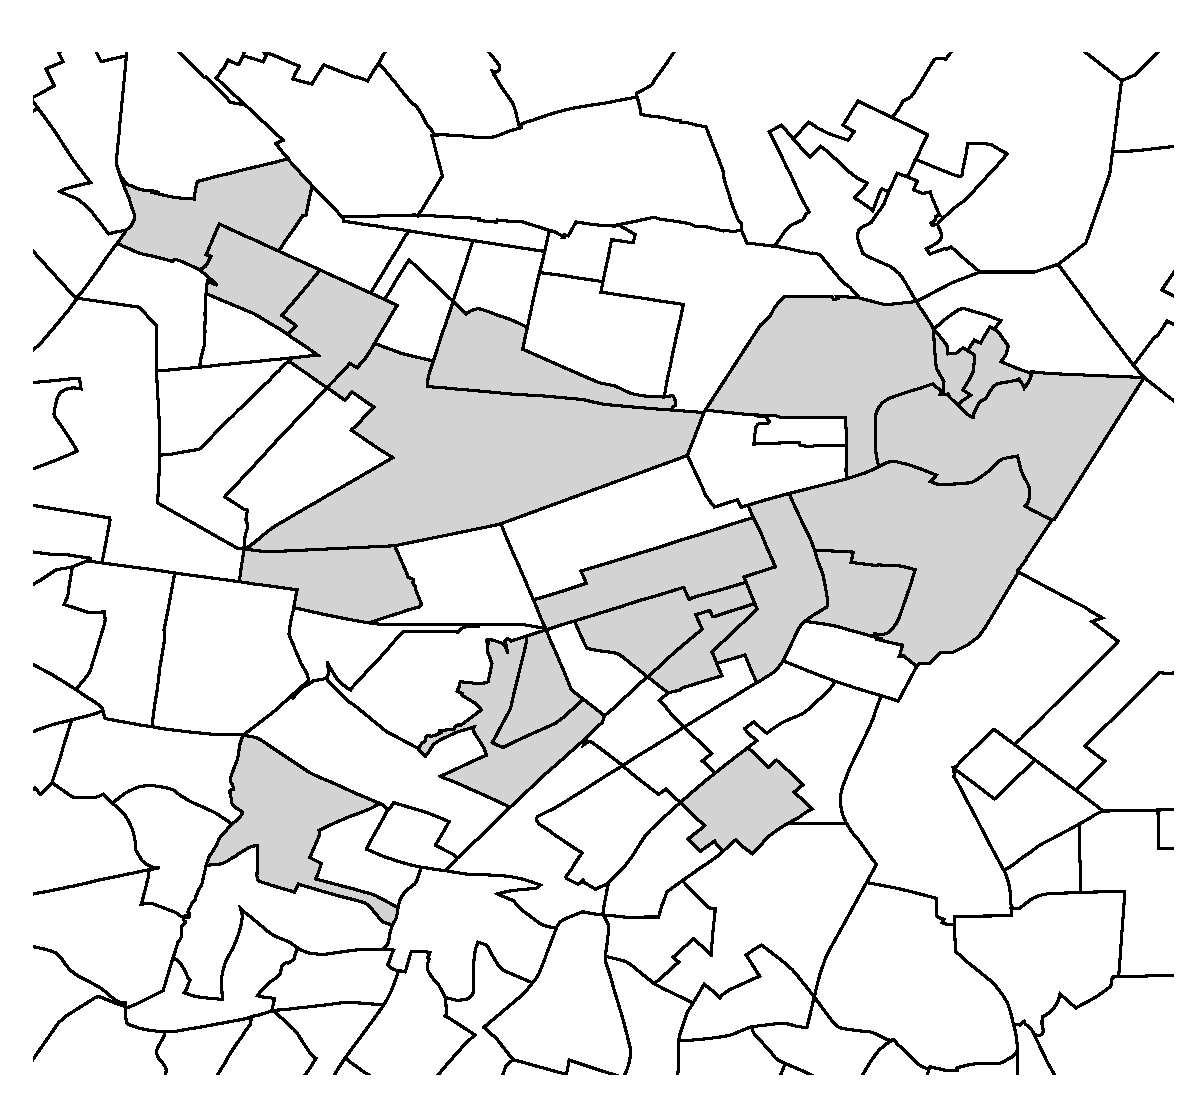
\includegraphics[width=0.75\textwidth]{gfx/chapter-monocentric/hotspots_boston.pdf}
    \caption{The census tracts of downtown Boston, MA in the US. In light grey,
    the census tracts that are identified as employment hotspots by the LouBar
method. Although the method designates all light grey tracts as different hotspots,
many of them are contiguous. We can wonder whether such contiguous
hotspots are, in fact, part of a larger hotspot that would include all of them.
This plot was generated with python, using the 2000 Census tract-to-tract
commuting flows and the 2000 Census tracts geometry.\label{fig:hotspots_boston}}
\end{figure}

This problem is in fact very general, and pertains to the field of spatial
analysis (including spatial statistics). Finding centers indeed amounts to
finding the proper way to describe a density profile at a meso-scale level and
to devising proper methods to detect the salient feature of this spatial
pattern. The tools provided by spatial analysis are however not yet suited to
provide such a description. This would however have huge potential applications.
With hindsight, such tools would also help to describe the spatial patterns of
segregation that we study in part \ref{part:stratification} of this
manuscript.

The results of the methods provided in the introduction should not be thrown
away altogether, though. The number of centers they provide probably does not
reflect the `real' number of centers (if there is such a thing) in a particular
city. But, assuming that different cities exhibit similar structures, they
should still provide values that are coherent across different urban areas, and
are thus useful for \emph{comparison} purposes.\\

\section{Summary}
\label{sec:summary}


In this part, we have presented an historical overview of the monocentric
hypothesis for the structure of cities, and how the view has progressively
shifted towards the picture of a more distributed, polycentric organisation.
Starting with indirect evidence for a polycentric picture, several methods were
then naturally proposed to directly measure the number of centers, from the
first parametric methods to the more recent non-parametric methods. Observing
evidence for an increased polycentricity with population size, we then wondered
what were the possible explanations for this phenomenon. We proposed an
out-of-equilibrium model of city growth that predicts the necessary emergence of
secondary centers as populations grows, and a sublinear increase of the number
of subcenters with population---both verified on empirical data, across
different countries, for several city definitions.

In the next part, we will continue our journey with another, seemingly unrelated
topic: scaling relationships. We will start with an historical perspective on
 scaling, showing that scaling relationships are older than most people believe,
 and we will provide a non-exhaustive review of the empirical results. We will
 then be ready to show how, using the model exposed in this chapter, we can
 understand the scaling relationships related to mobility in cities. We will
 then conclude on a reflection of what scaling relationships can and do tell us about cities,
 and highlight their shortcomings.



